\documentclass[tikz,border=10pt]{standalone}
\usepackage{tikz}
\usetikzlibrary{positioning, fit, arrows.meta, shapes, backgrounds}

\begin{document}
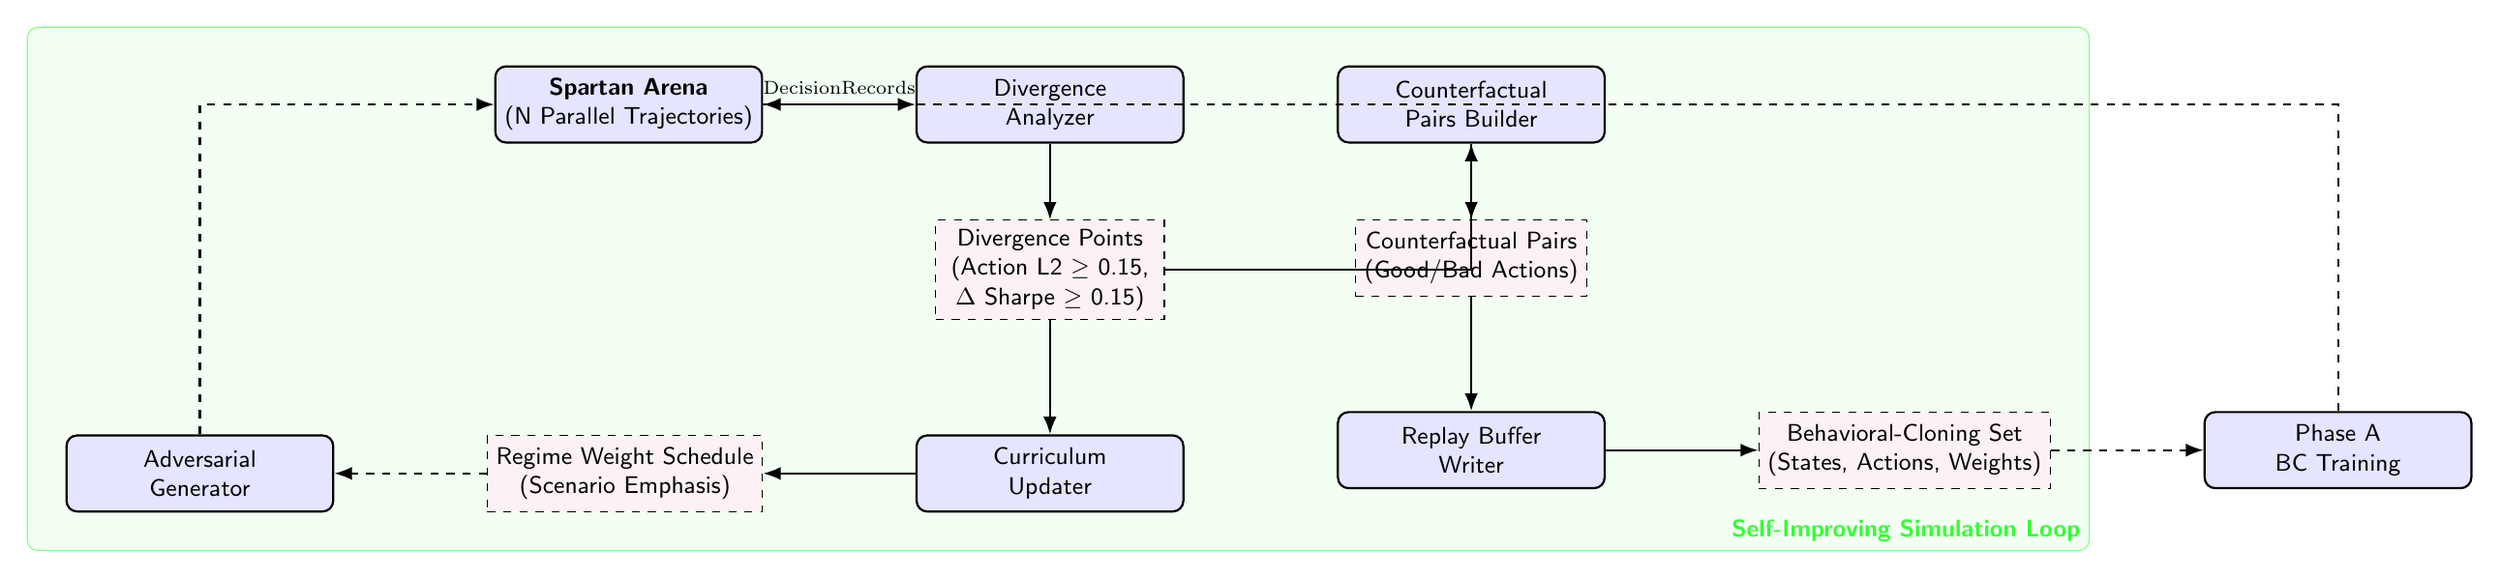
\begin{tikzpicture}[
    font=\sffamily\small,
    >=LaTeX,
    process/.style={rectangle, rounded corners, draw, thick, fill=blue!10, minimum width=3.5cm, minimum height=1cm, align=center},
    evidencebox/.style={rectangle, draw, dashed, fill=purple!5, minimum width=3cm, minimum height=1cm, align=center},
    db/.style={cylinder, draw, thick, shape border rotate=90, aspect=0.25, fill=gray!10, minimum width=2.5cm, minimum height=1.2cm, align=center},
    arrow/.style={->, thick},
    dashed_arrow/.style={->, thick, dashed}
]

% Nodes
\node[process] (arena) {\textbf{Spartan Arena} \\ (N Parallel Trajectories)};
\node[process, right=2cm of arena] (div_analyzer) {Divergence \\ Analyzer};
\node[evidencebox, below=1cm of div_analyzer] (div_points) {Divergence Points \\ (Action L2 $\ge$ 0.15, \\ $\Delta$ Sharpe $\ge$ 0.15)};

\node[process, right=2cm of div_analyzer] (cf_builder) {Counterfactual \\ Pairs Builder};
\node[evidencebox, below=1cm of cf_builder] (cf_pairs) {Counterfactual Pairs \\ (Good/Bad Actions)};

\node[process, below=1.5cm of div_points] (updater) {Curriculum \\ Updater};
\node[evidencebox, left=2cm of updater] (curriculum_cfg) {Regime Weight Schedule \\ (Scenario Emphasis)};

\node[process, below=1.5cm of cf_pairs] (bc_writer) {Replay Buffer \\ Writer};
\node[evidencebox, right=2cm of bc_writer] (bc_dataset) {Behavioral-Cloning Set \\ (States, Actions, Weights)};

\node[process, left=2cm of curriculum_cfg] (adv_gen) {Adversarial \\ Generator};
\node[process, right=2cm of bc_dataset] (bc_train) {Phase A \\ BC Training};

% Connections
\draw[arrow] (arena) -- node[above, font=\scriptsize] {DecisionRecords} (div_analyzer);
\draw[arrow] (div_analyzer) -- (div_points);
\draw[arrow] (div_points) -| (cf_builder);
\draw[arrow] (cf_builder) -- (cf_pairs);

\draw[arrow] (div_points) -- (updater);
\draw[arrow] (cf_pairs) -- (bc_writer);

\draw[arrow] (updater) -- (curriculum_cfg);
\draw[arrow] (bc_writer) -- (bc_dataset);

\draw[dashed_arrow] (curriculum_cfg) -- (adv_gen);
\draw[dashed_arrow] (adv_gen) |- (arena);

\draw[dashed_arrow] (bc_dataset) -- (bc_train);
\draw[dashed_arrow] (bc_train) |- (arena);

\begin{scope}[on background layer]
    \node[draw=green!50, fill=green!5, rounded corners, fit=(adv_gen)(arena)(div_analyzer)(cf_builder)(div_points)(cf_pairs)(updater)(curriculum_cfg)(bc_writer)(bc_dataset), inner sep=0.5cm] (loop_bg) {};
    \node[above left, text=green!80] at (loop_bg.south east) {\textbf{Self-Improving Simulation Loop}};
\end{scope}

\end{tikzpicture}
\end{document}
